\documentclass{article}

% Useful packages
\usepackage{multicol}
\setlength{\columnsep}{1cm}

% Set page size and margins
% Replace `letterpaper' with `a4paper' for UK/EU standard size
\usepackage[a4paper,top=2cm,bottom=2cm,left=2cm,right=2cm,marginparwidth=1.75cm]{geometry}

\usepackage{caption}
\usepackage{amsmath}
\usepackage{siunitx}
\usepackage{wrapfig}
\usepackage{float}
\usepackage{graphicx}
\graphicspath{{metingen/}}
\usepackage{subcaption}
\usepackage[colorlinks=true, allcolors=blue]{hyperref}
\usepackage{xcolor}
\usepackage{listings}
\usepackage{import}
\usepackage{xcolor}

% Definieer de kleuren voor syntax highlighting
\definecolor{codegreen}{rgb}{0,0.6,0}
\definecolor{codegray}{rgb}{0.5,0.5,0.5}
\definecolor{codepurple}{rgb}{0.58,0,0.82}
\definecolor{backcolour}{rgb}{0.95,0.95,0.92}

\lstdefinestyle{mystyle}{
    backgroundcolor=\color{backcolour},
    commentstyle=\color{codegreen},
    keywordstyle=\color{codepurple},
    numberstyle=\tiny\color{codegray},
    basicstyle=\footnotesize\ttfamily,
    breakatwhitespace=false,
    breaklines=true,
    captionpos=b,
    keepspaces=true,
    numbers=left,
    numbersep=5pt,
    showspaces=false,
    showstringspaces=false,
    showtabs=false,
    tabsize=2
}

\usepackage[dutch]{babel}% Language setting


\title{Hardware Implementatie Overspraakproef}

\author{
  Vollmuller, Michel\\
  1809572\\
  \texttt{michel.vollmuller@student.hu.nl}
  \and
  Willems, Tijmen\\
  1805057\\
  \texttt{tijmen.willems@student.hu.nl}
}

\begin{document}
\maketitle

\begin{abstract}
    Hier komt een mooie abstract
\end{abstract}

\tableofcontents

\newpage

\section{Inleiding}
\begin{figure}[H]
    \centering
    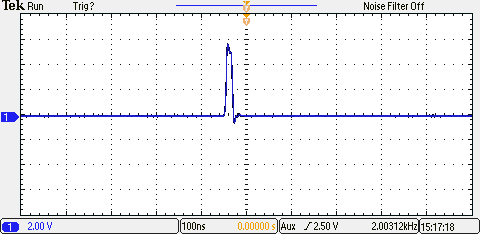
\includegraphics[scale=0.5]{geen kabel.PNG}
    \caption{geen kabel}
    \label{fig:geen kabel}
\end{figure}

\newpage

\section{Meetrapport}
\subsection{Open Uiteinde}
\begin{itemize}
    \item Verwachting\\
    Wanneer een kabel is aangesloten met een open einde zouden er reflecties plaatsvinden in fase.
    \item Meeting
    \begin{figure}[H]
        \centering
        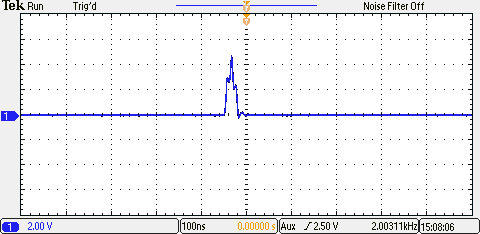
\includegraphics[scale=0.5]{open uiteinde.PNG}
        \caption{meting open uiteinde}
        \label{fig:meting open uiteinde}
    \end{figure}
    \item Evaluatie\\
    In afbeelding \ref{fig:meting open uiteinde} is duidelijk het signaal van de functie generator te zien + de reflectie die in fase plaatsvindt.
\end{itemize}

\subsection{Gesloten uiteinde}
\begin{itemize}
    \item Verwachting\\
    Wanneer een kabel is aangesloten met een geslote einde zouden er reflecties plaatsvinden in tegenfase.
    \item Meeting
    \begin{figure}[H]
        \centering
        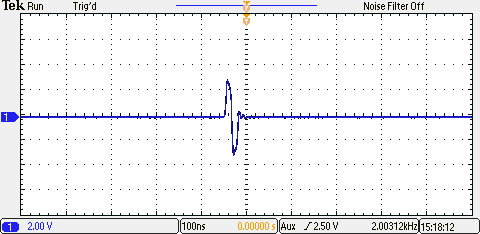
\includegraphics[scale=0.5]{gesloten uiteinde.PNG}
        \caption{meting gesloten uiteinde}
        \label{fig:meting gesloten uiteinde}
    \end{figure}
    \item Evaluatie\\
    In afbeelding \ref{fig:meting gesloten uiteinde} is duidelijk het signaal van de functie generator te zien + de reflectie die in tegenfase plaatsvindt.
\end{itemize}

\subsection{Karakteristiek afgesloten 50 ohm}
\begin{itemize}
    \item Verwachting\\
    Met een karakteristiek afgelsoten kabel zou er geen reflectie moeten plaatsvinden. Waarbij je dan dus alleen het originele signaal zou moeten zien.
    \item Meeting
    \begin{figure}[H]
        \centering
        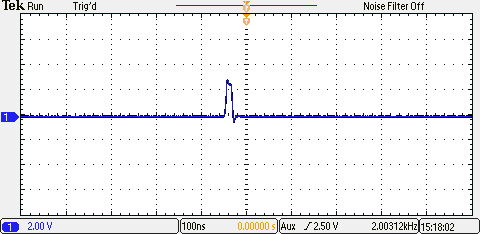
\includegraphics[scale=0.5]{50ohm termination.PNG}
        \caption{meting karakteristiek afgesloten}
        \label{fig:meting karakteristiek afgesloten}
    \end{figure}
    \item Evaluatie\\
    In afbeelding \ref{fig:meting karakteristiek afgesloten} is duidelijk het signaal van de functie generator te zien doordat hij karakteristiek is afgesloten. Echter is ook te zien dat de amplitude de helft is van het orignele signaal. Dit komt doordat er een spanningsdeling plaatsvind door de weerstand van de functiegenerator en de termination.
\end{itemize}

\subsection{lengte coax kabel}
Het aanpassen van de bronweerstand is niet nodig, omdat je de kabel ook niet afsluit met een termination weerstand.

\hspace{1cm}\\
\\
Vanwege die weerstand is de snelheid in onafgeschermd koper ongeveer 96\% van de lichtsnelheid, maar in een typische coaxkabel (antennesnoer) is het ongeveer 66\% van de lichtsnelheid. 
% Even een bronnetje teovoegen https://www.rijnmond.nl/nieuws/97527/hoe-snel-gaat-elektriciteit
Door te meten hoelang het duurt voordat er een reflectie plaatsvind kan je met deze tijd bereken hoelang de kabel is.

\begin{figure}[H]
    \centering
    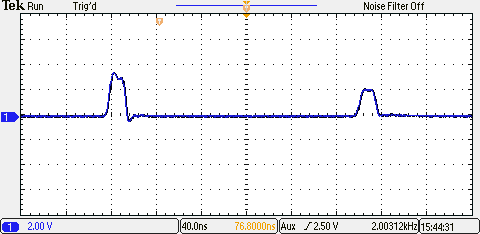
\includegraphics[scale=0.5]{reflectie rol coax.PNG}
    \caption{reflectie rol coax}
    \label{fig:reflectie rol coax}
\end{figure}

In afbeelding \ref{fig:reflectie rol coax} is te zien dat de reflectie optreed na ongeeveer $220\cdot10^{-9}$ met deze info kan de lengte van de kabel berekend worden.

\begin{equation}
    \begin{split}
        lengte &= \frac{c \cdot 0,66 \cdot 220\cdot10^{-9}}{2}\\
        &\Downarrow \\
         &= 21,76m
    \end{split}
\end{equation}



%Bibliography
% \bibliographystyle{IEEEtran}
% \bibliography{bib}
% \appendix

% \bibliographystyle{IEEEtran}
% \bibliography{bib}

\end{document}